\documentclass{beamer}

\usetheme{default}
\usecolortheme{default}

\title{The Waterfall Method}

\author{Lucas JACQUIN, Corentin MENGEL, Vincent ITALIANO, Antoine SCHUFFENECKER, Abdelhamid MOLTAZIM}

\begin{document}
\begin{frame}    
    
    \maketitle

\end{frame}

\begin{frame}
    \frametitle{Introduction and history}
    \begin{itemize}
        \setlength\itemsep{1em}
        \item First design model in Software Engineering \pause
        \item Originates from construction and manufacturing industries \\
        \quad\quad$\Rightarrow$ prevent costly design changes\pause
        \item Activities in sequential phases \pause
        \item Earliest use of such phases was in 1956 (SAGE) \pause
        \item Term "waterfall" firstly used in a 1976 paper \pause
        \item Made into a standard by the US Department of Defense in 1985.
    \end{itemize}
\end{frame}

\begin{frame}
    \frametitle{Phases of waterfall project management}
    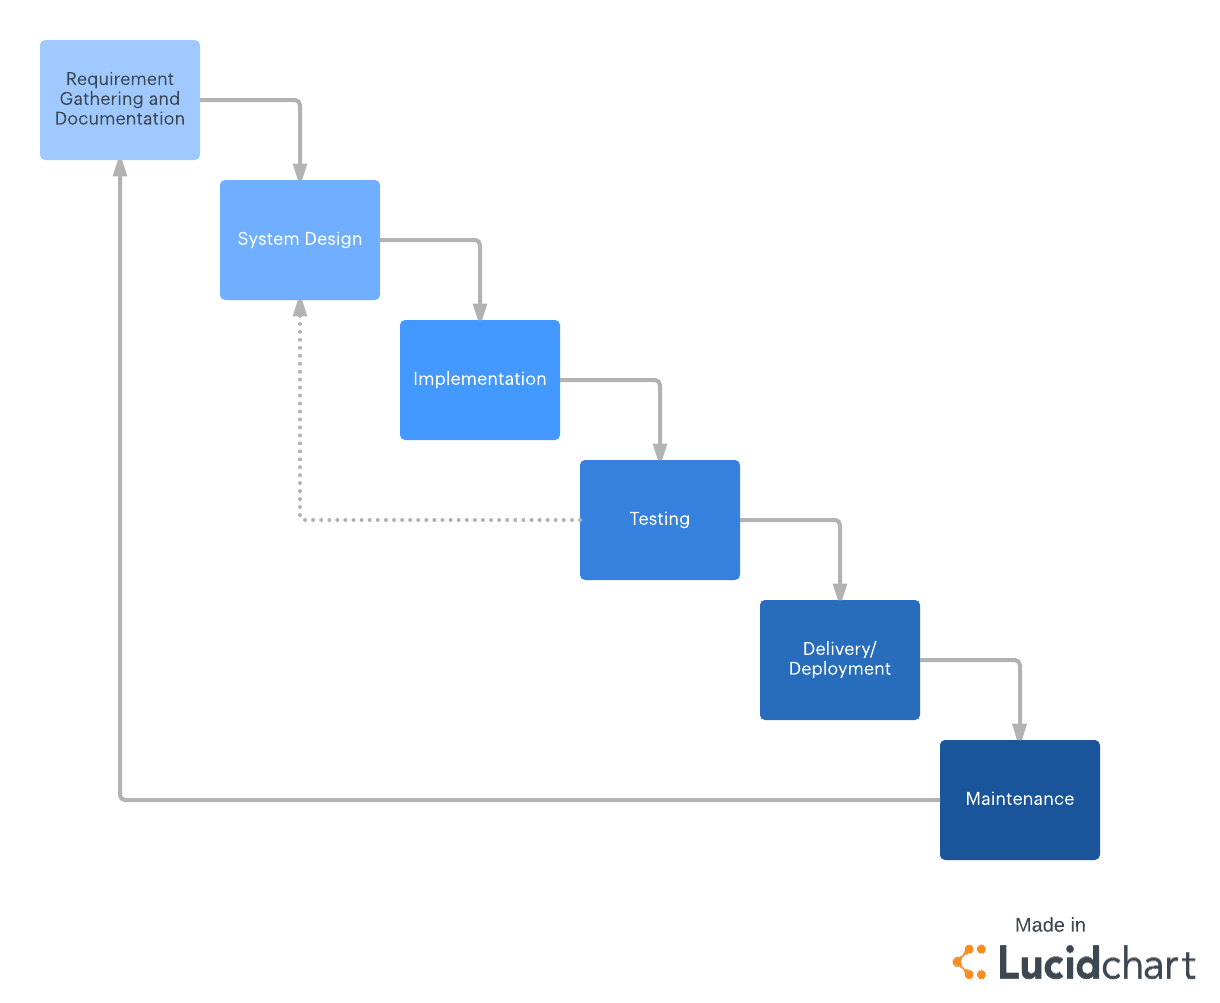
\includegraphics[scale=0.25]{Images/WaterfallDiagram.png}
\end{frame}

\begin{frame}
    \frametitle{Phases of waterfall project management}
    \begin{itemize}
        \setlength\itemsep{1em}
        \item Requirement gathering and documentation \pause
        \item System design \pause
        \item Implementation \pause
        \item Testing \pause
        \item Delivery/deployment \pause
        \item Maintenance
    \end{itemize}
\end{frame}

\begin{frame}
    \frametitle{Examples of waterfall project management}
    \begin{itemize}
        \setlength\itemsep{1em}
        \item Energy management systems for electrical utilities \pause
        \item Rail traffic control systems for railways \pause
        \item Information systems infrastructure \pause
        \item Customer relationship management systems \pause
        \item Human resource management systems \pause
        \item Inventory management systems     
    \end{itemize}
\end{frame}

\begin{frame}
    
    \frametitle{The PROS and CONS of the Waterfall project management}
    \begin{itemize}
    \begin{columns}[T] % align columns
        \begin{column}{.48\textwidth}
        PROS \pause
        \item Simple 
        \item Easy to implement 
        \item Logical 
        \item Organized 
        \item Estimation of the costs 
        \end{column}%
        \hfill%
        \begin{column}{.48\textwidth}
        CONS \pause
        \item Not Flexible
        \item Fail to satisfy expectations 
        \item Vulnerabilities to changes and unexpected events
        \end{column}%
        \end{columns}   
        \setlength\itemsep{1em}
        
        
    \end{itemize}
\end{frame}

\nocite{*}
\begin{frame}
    \frametitle{Bibliography}

    \bibliographystyle{plain}
    {\footnotesize
    \bibliography{waterfall}}

\end{frame}

\end{document}
